\documentclass{sigchi}

% Use this section to set the ACM copyright statement (e.g. for
% preprints).  Consult the conference website for the camera-ready
% copyright statement.

% Copyright
\CopyrightYear{2016}
%\setcopyright{acmcopyright}
\setcopyright{acmlicensed}
%\setcopyright{rightsretained}
%\setcopyright{usgov}
%\setcopyright{usgovmixed}
%\setcopyright{cagov}
%\setcopyright{cagovmixed}
% DOI
\doi{http://dx.doi.org/10.475/123_4}
% ISBN
\isbn{123-4567-24-567/08/06}
%Conference
\conferenceinfo{CHI'16,}{May 07--12, 2016, San Jose, CA, USA}
%Price
\acmPrice{\$15.00}

% Use this command to override the default ACM copyright statement
% (e.g. for preprints).  Consult the conference website for the
% camera-ready copyright statement.

%% HOW TO OVERRIDE THE DEFAULT COPYRIGHT STRIP --
%% Please note you need to make sure the copy for your specific
%% license is used here!
% \toappear{
% Permission to make digital or hard copies of all or part of this work
% for personal or classroom use is granted without fee provided that
% copies are not made or distributed for profit or commercial advantage
% and that copies bear this notice and the full citation on the first
% page. Copyrights for components of this work owned by others than ACM
% must be honored. Abstracting with credit is permitted. To copy
% otherwise, or republish, to post on servers or to redistribute to
% lists, requires prior specific permission and/or a fee. Request
% permissions from \href{mailto:Permissions@acm.org}{Permissions@acm.org}. \\
% \emph{CHI '16},  May 07--12, 2016, San Jose, CA, USA \\
% ACM xxx-x-xxxx-xxxx-x/xx/xx\ldots \$15.00 \\
% DOI: \url{http://dx.doi.org/xx.xxxx/xxxxxxx.xxxxxxx}
% }

% Arabic page numbers for submission.  Remove this line to eliminate
% page numbers for the camera ready copy
% \pagenumbering{arabic}

% Load basic packages
\usepackage{balance}       % to better equalize the last page
\usepackage{graphics}      % for EPS, load graphicx instead 
\usepackage[T1]{fontenc}   % for umlauts and other diaeresis
\usepackage{txfonts}
\usepackage{mathptmx}
\usepackage[pdflang={en-US},pdftex]{hyperref}
\usepackage{color}
\usepackage{booktabs}
\usepackage{textcomp}
\usepackage{svg}
\usepackage{pdfpages}

% Some optional stuff you might like/need.
\usepackage{microtype}        % Improved Tracking and Kerning
% \usepackage[all]{hypcap}    % Fixes bug in hyperref caption linking
\usepackage{ccicons}          % Cite your images correctly!
% \usepackage[utf8]{inputenc} % for a UTF8 editor only

% If you want to use todo notes, marginpars etc. during creation of
% your draft document, you have to enable the "chi_draft" option for
% the document class. To do this, change the very first line to:
% "\documentclass[chi_draft]{sigchi}". You can then place todo notes
% by using the "\todo{...}"  command. Make sure to disable the draft
% option again before submitting your final document.
\usepackage{todonotes}

% Paper metadata (use plain text, for PDF inclusion and later
% re-using, if desired).  Use \emtpyauthor when submitting for review
% so you remain anonymous.
\def\plaintitle{Intelligent Monitoring for Detecting Semantic Misalignment Between Promotion Links and Landing Pages}
\def\plainauthor{First Author, Second Author, Third Author,
  Fourth Author, Fifth Author, Sixth Author}
\def\emptyauthor{}
\def\plainkeywords{Authors' choice; of terms; separated; by
  semicolons; include commas, within terms only; required.}
\def\plaingeneralterms{Documentation, Standardization}

% llt: Define a global style for URLs, rather that the default one
\makeatletter
\def\url@leostyle{%
  \@ifundefined{selectfont}{
    \def\UrlFont{\sf}
  }{
    \def\UrlFont{\small\bf\ttfamily}
  }}
\makeatother
\urlstyle{leo}


% To make various LaTeX processors do the right thing with page size.
\def\pprw{8.5in}
\def\pprh{11in}
\special{papersize=\pprw,\pprh}
\setlength{\paperwidth}{\pprw}
\setlength{\paperheight}{\pprh}
\setlength{\pdfpagewidth}{\pprw}
\setlength{\pdfpageheight}{\pprh}

% Make sure hyperref comes last of your loaded packages, to give it a
% fighting chance of not being over-written, since its job is to
% redefine many LaTeX commands.
\definecolor{linkColor}{RGB}{6,125,233}
\hypersetup{%
  pdftitle={\plaintitle},
% Use \plainauthor for final version.
%  pdfauthor={\plainauthor},
  pdfauthor={\emptyauthor},
  pdfkeywords={\plainkeywords},
  pdfdisplaydoctitle=true, % For Accessibility
  bookmarksnumbered,
  pdfstartview={FitH},
  colorlinks,
  citecolor=black,
  filecolor=black,
  linkcolor=black,
  urlcolor=linkColor,
  breaklinks=true,
  hypertexnames=false
}

% create a shortcut to typeset table headings
% \newcommand\tabhead[1]{\small\textbf{#1}}

% End of preamble. Here it comes the document.
\begin{document}

\title{\plaintitle}

\numberofauthors{3}
\author{%
  \alignauthor{Leave Authors Anonymous\\
    \affaddr{for Submission}\\
    \affaddr{City, Country}\\
    \email{e-mail address}}\\
  \alignauthor{Leave Authors Anonymous\\
    \affaddr{for Submission}\\
    \affaddr{City, Country}\\
    \email{e-mail address}}\\
  \alignauthor{Leave Authors Anonymous\\
    \affaddr{for Submission}\\
    \affaddr{City, Country}\\
    \email{e-mail address}}\\
}

\maketitle

\begin{abstract}
  Hyperlinks must always work and direct to relevant landing pages. While document owners are responsible for the quality of links, no existing tools support efficient, accurate, and timely testing of link relevance. This paper reports how we developed an intelligent monitoring agent focusing on promotion emails. First, we identify eight types of misalignment that people commonly perceive from promotion emails. We then collect ground-truth labels of link relevance, and find the best performing model from a wide range of relevance metrics including deep neural networks. Finally we introduce the monitoring agent, which takes emails as input, periodically monitors content of linked pages, estimates semantic relevance between each pair of link and landing pages, and allows marketers to overview current status of their emails and potential misalignments. Initial feedback from marketers in a longitudinal case study suggests that our system will provide benefits to email marketers. 
\end{abstract}

\category{H.5.m.}{Information Interfaces and Presentation
  (e.g. HCI)}{Miscellaneous} 
  %\category{See\url{http://acm.org/about/class/1998/} for the full list of ACM classifiers. This section is required.}{}{}

\keywords{Promotional email; Link relevance; Deep learning; Interactive system 
%\plainkeywords
}

\section{Introduction}
Hyperlinks are what make online documents truly meaningful. A successful link must take users to the page with relevant content. However, it is not uncommon to see people getting confused or disappointed by error messages or unexpected content on landing pages. A promotion link, for instance, can be misaligned in many ways, as illustrated in Figure~\ref{fig:shoes}. Such misalignments might lose not only immediate business opportunities but also long-term relationship with customers. However, to the best of our knowledge, existing tools can only detect dead links, leaving subtle semantic misalignments to marketer's inefficient, inaccurate, and belated manual testing. Our goal in this paper is to make link testing an efficient, accurate, and timely task for marketers. 

Perception of link misalignment is subjective and contextual. In other words, even if marketers believe their links are relevant with landing pages, some people may not agree. Therefore, to extend our understanding of the problem we conducted an online survey with 211 participants recruited from Amazon Mechanical Turk (MTurk), and identify eight types of misalignments in this paper. We discuss about two high-level reasons behind misalignments: mismatch between static email and dynamic web, and the gap between marketer and customer mindset. 

The key component of our system is the metric that automatically estimates whether a pair of link and landing page is misaligned. To the best of our knowledge, there exists no labeled dataset for training or validating the relevance metric. We conducted an online experiment using MTurk that collects five labels for each of 4266 links. Results suggest that 58.1\% of the links are perceived to be misaligned by at least one out of five people. 4.8\% of links are perceived to be misaligned by all five people.          

We provide a brief exploratory study where we compare unsupervised baseline models and artificial neural networks for predicting misalignment. The unsupervised approaches achieve an F-score of 0.74 and 0.48 for the settings where at least one and, respectively, where at least three persons identify a misalignment; the neural networks achieve 0.76 and 0.66.

Lastly, we present an intelligent monitoring agent that enables marketers to efficiently monitor relevance of links in their promotion emails. The process begins when a marketer registering an email to our system. It extracts all the links within the email, and starts retrieving content on the landing pages periodically. If the relevance metric estimates a link to be misaligned, the agent notifies the marketer via email or other channels. The marketer can see the overview of all his/her emails and latest report. 

The main contributions of this paper are summarized as follows.
\begin{itemize}
\item An online survey that identifies types of misalignments between promotion links and landing pages. 
\item A labeled dataset that contains misalignments of 4266 links extracted from 160 emails. Each link received five votes of perceived misalignments. 
\item A novel link relevance metric that estimates how relevant a pair of link and its landing page is.  
\item An experimental result that compared artificial neural networks and unsupervised baseline models.


\item A novel end-to-end interactive system for monitoring link relevance. The system includes components of the entire information pipeline: HTML parsing, indexing, landing page crawling, relevance metric, and a web portal for managing registered emails and relevance reports. 
\end{itemize}

\begin{figure}
\centering
  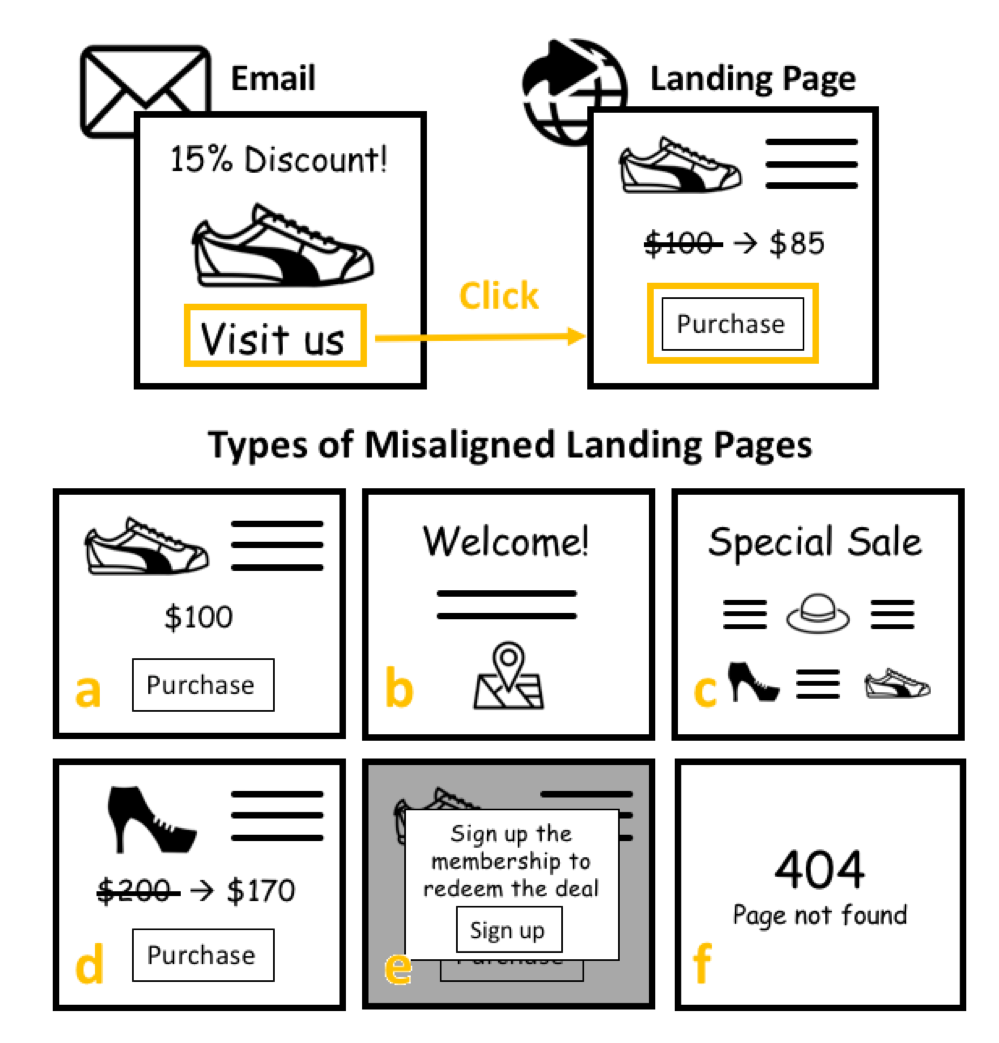
\includegraphics[width=0.75\columnwidth]{figures/types}
  \caption{A successful marketing email must be relevant to its landing pages. However, there exist many cases of misalignments including (a) expired offering, redirected to (b) domain root page or (c) other irrelevant pages, (d) showing unrelated content, (e) asking for unexpected steps such as sign-up, (e) showing error pages.}~\label{fig:shoes}
\end{figure}


% ██████╗ ███████╗██╗      █████╗ ████████╗███████╗██████╗ 
% ██╔══██╗██╔════╝██║     ██╔══██╗╚══██╔══╝██╔════╝██╔══██╗
% ██████╔╝█████╗  ██║     ███████║   ██║   █████╗  ██║  ██║
% ██╔══██╗██╔══╝  ██║     ██╔══██║   ██║   ██╔══╝  ██║  ██║
% ██║  ██║███████╗███████╗██║  ██║   ██║   ███████╗██████╔╝
% ╚═╝  ╚═╝╚══════╝╚══════╝╚═╝  ╚═╝   ╚═╝   ╚══════╝╚═════╝ 
                                                         
% ██╗    ██╗ ██████╗ ██████╗ ██╗  ██╗                      
% ██║    ██║██╔═══██╗██╔══██╗██║ ██╔╝                      
% ██║ █╗ ██║██║   ██║██████╔╝█████╔╝                       
% ██║███╗██║██║   ██║██╔══██╗██╔═██╗                       
% ╚███╔███╔╝╚██████╔╝██║  ██║██║  ██╗                      
%  ╚══╝╚══╝  ╚═════╝ ╚═╝  ╚═╝╚═╝  ╚═╝  
\section{Related Work}
\subsubsection{Broken links on the Internet}
The death and decay of web references is a well-known phenomenon studied by many researchers. Fetterly et al. \cite{fetterly_large-scale_2003} observed that pages disappear at a rate of 0.25-0.5\% per week. Hennessey and Ge \cite{hennessey_cross_2013} found out that the median lifespan of hyperlinks used in scientific literature was 9.3 years. Zittrain et al. \cite{zittrain_perma:_2014} have determined that approximately 50\% of the URLs in U.S. Supreme Court opinions no longer link to the original information. While determining a dead link is relatively easy by checking the 404 "Page Not Found" error code, many web servers redirects users to alternative (but completely different from the original) pages, and return 200 Ok codes - called "soft-404s" \cite{bar-yossef_sic_2004}. There are many tools that detect hard-404s. For instance, W3C Link Checker\footnote{https://validator.w3.org/checklink} tests all the links in a HTML document landing page direct to valid landing pages. Email marketing platforms such as Adobe Campaign, Litmus, and DotMailer provide features for testing whether URLs within an email are reachable. To our knowledge, however, there is no tool for detecting subtle semantic misalignments. 

\subsubsection{Improving online marketing with technology}
Improving the effectiveness of online marketing has been a popular research topic for machine learning researchers. For example, contextual matching aims to provide ads that are closely related with the user's current interest and the pages where the ads are shown on. Chakrabarti et al\cite{chakrabarti2008contextual} proposed a logistic regression model to determine relevancy of ads and landing pages to show them on. Another line of research tries to predict click rate of ads using clustering, keyword matching, and classification in the context of sponsored search \cite{regelson2006predicting}. Becker et al \cite{Becker:2009:HAA:1645953.1645964} analyzed the impact of a landing page on the user's conversion behavior for different advertisement categories in the context of sponsored search. Rosales et al.\cite{Rosales:2012:PCM:2124295.2124333} proposed a model to estimate a conversion rate after users click promotion links. While the aforementioned work on online advertising focuses on the relevancy of ad itself, but not semantic relevance of links and landing pages. 

\subsubsection{Metrics for link relevance}
To our best knowledge, there is not much prior work directly modeling the semantic similarity between links and landing pages. One of the closest metrics would be similarity measures, which have been used for various applications such as document clustering \cite{huang2008similarity}, summarization, plagiarism detection \cite{lukashenko2007computer}, and creating anchor text from a target document  \cite{rebervsek-verlic:2013:EMNLP}. Gong et al.\,\cite{Gong:2017:MLW:3123266.3123296} leveraged both image and text information on the web page to improve information extraction results. Similarly, we extracted tags and metadata from images on promotional emails using OCR and image recognition algorithms to extract more semantic features. Bylinskii et al. \cite{Bylinskii:2017:LVI:3126594.3126653} learned automated models to predict relative importance of different elements in data visualizations and graphic designs. Our work is to develop a method to predict the semantic relevance of links. 



% ███╗   ███╗██╗███████╗ █████╗ ██╗     ██╗ ██████╗ ███╗   ██╗███╗   ███╗███████╗███╗   ██╗████████╗███████╗
% ████╗ ████║██║██╔════╝██╔══██╗██║     ██║██╔════╝ ████╗  ██║████╗ ████║██╔════╝████╗  ██║╚══██╔══╝██╔════╝
% ██╔████╔██║██║███████╗███████║██║     ██║██║  ███╗██╔██╗ ██║██╔████╔██║█████╗  ██╔██╗ ██║   ██║   ███████╗
% ██║╚██╔╝██║██║╚════██║██╔══██║██║     ██║██║   ██║██║╚██╗██║██║╚██╔╝██║██╔══╝  ██║╚██╗██║   ██║   ╚════██║
% ██║ ╚═╝ ██║██║███████║██║  ██║███████╗██║╚██████╔╝██║ ╚████║██║ ╚═╝ ██║███████╗██║ ╚████║   ██║   ███████║
% ╚═╝     ╚═╝╚═╝╚══════╝╚═╝  ╚═╝╚══════╝╚═╝ ╚═════╝ ╚═╝  ╚═══╝╚═╝     ╚═╝╚══════╝╚═╝  ╚═══╝   ╚═╝   ╚══════╝

\section{Identifying Types of Misalignments}
To extend our understanding of misalignments between promotion links and landing pages, we conducted an online survey. 

\subsection{Method}
The survey was posted it on MTurk for workers living in the United States. We paid \$0.3 for each participation. First of all, we requested participants to open their inboxes for automatically-classified promotion emails. They estimated average numbers of daily promotion emails received and opened. They then picked multiples among important factors (Targeted offer, Value of the offer, Brand image, Trustworthiness, Limited-time offer) considered when opening emails, and/or describing their own reasons. Lastly they looked for misaligned links by following the instruction, \textit{``We are collecting promotion emails whose link do not consistent with linked pages. Open a promotion email that you received recently. Click a few links, and check their landing pages are matching. Are they all matching? If yes, open another email, and repeat the same process until you find a landing page irrelevant to its link''}. For an email containing a misaligned link, each participant provided the email's subject, sender, link text, and the reason why he/she perceived the link to be irrelevant. They also rated the negative impact of the misalignment to the campaign.


%%%%%  FIGURES ABOUT THE ONLINE SURVEY
\begin{figure}
\centering
  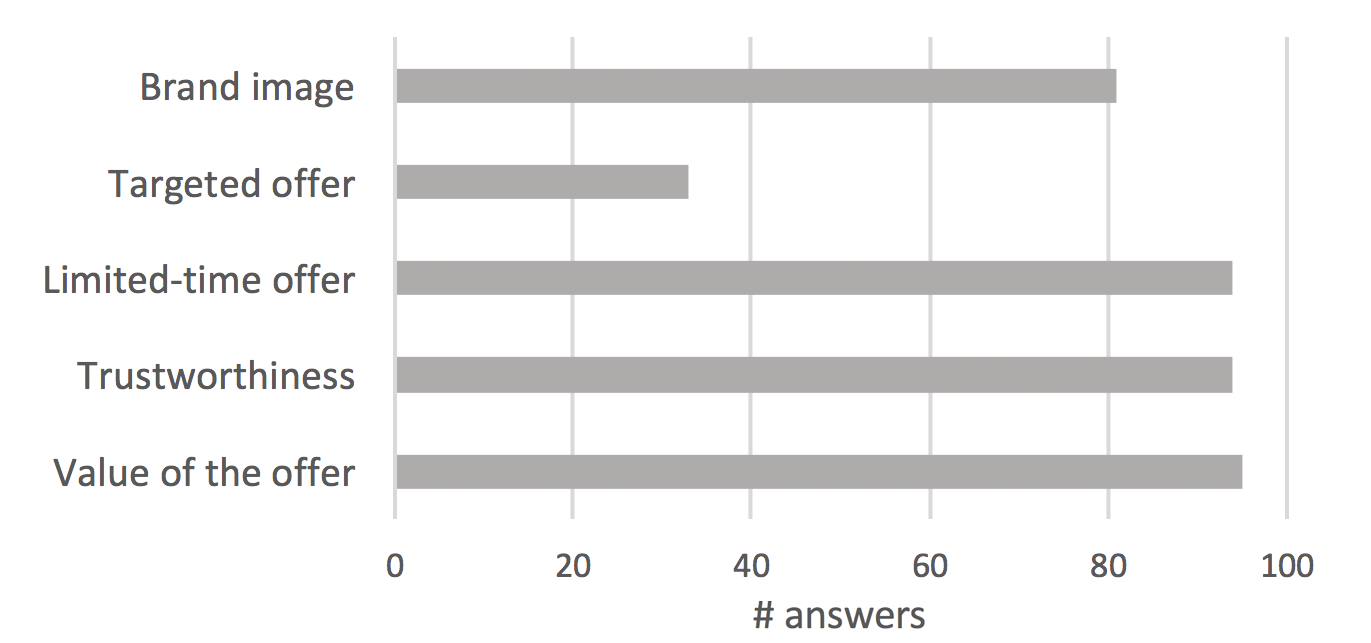
\includegraphics[width=0.85\columnwidth]{figures/open-email-factors}
  \caption{Factors that participants consider when opening a promotion email}~\label{fig:open-email-factors}
\end{figure}

\subsection{Result}
211 participants recruited from MTurk for two days. Participants tends to be young, well-educated, and female, with moderately high incomes according to prior research about general demographic of MTurk \cite{mason_conducting_2012}. The majority of participants daily receive 1-20 promotion emails (AVG: 17.4), and open 0-5 emails (AVG: 10.6). As illustrated in Figure~\ref{fig:open-email-factors}, Targeted offer turns out to be the least important factor among five options for opening promotion emails. Although we did not give them specific point stop, participants checked average 7.3 emails until they found a misalignment or stopped searching. Among 211 participants, 160 (75\%) participants found emails containing at least one misalignment, while 51 (24\%) finished the survey without finding any misalignment. Despite the given instruction, 59 participants reported issues that are about emails rather than links. For instance, 31 (15\%) participants reported uninteresting or irrelevant emails. 28 (13\%) participants reported fake or spam information in their emails. In the following section we focus on the rest - 101 (48\%) cases of misalignments between links and their landing pages. 


\subsection{Types of Misalignments}
The first author reviewed the 101 cases misalignments focusing on the reason why the participant thought the link and the landing page are misaligned. Through iterative coding, we identified eight common patterns of misalignments, ordered by frequency. 
\subsubsection{T1. Irrelevant page}
29 (14\%) participants reported landing pages that are entirely irrelevant with the links. They said, \textit{``It has nothing to do with my initial email''} (P30), \textit{``It took me to a page of Microsoft Surface devices, not office equipment''} (P32), \textit{``Page jumps to outlet store locations, not the group containing the sales''} (P25), and \textit{``It was labeled privacy policy but took me to unsubscribe page''} (P22). Most of those cases appear to be maintenance issues on the landing pages, but we could not find any further clue. 
\subsubsection{T2. Missing offer}
16 (8\%) participants reported that expected offers were missing even though the pages itself seem correct. For instance, "There is no hotels half off!" (P17), and "Does not take me to promo codes" (P53). While exact reasons may vary, many cases of T2 were limited-time offers that had expired already.  
\subsubsection{T3. Unexpected steps}
16 (8\%) participants reported landing pages that require them to do survey, subscription, quiz, or sharing on social media. For instance, P75 said, \textit{``It leads to something that wants me to advertise them on social media.''} Unexpected steps are often followed by missing offers (T2) as P53 said, \textit{``It took me to a page that began a bunch of surveys and 'offers', but I never got to a place to request Febreze samples.''} 
\subsubsection{T4. Fail to open landing page}
12 (6\%) participants found emails whose landing pages could not be loaded. In specific, 6 cases were web browser's errors such as \textsf{\small 404 Page Not Found}, \textsf{\small 400 Bad Request}, or \textsf{\small Corrupted Content Error}. Three were soft-404s, which are custom error pages of the servers, and another three were completely empty pages. 
\subsubsection{T5. Showing domain root}
9 (4\%) participants reported that promotion links took them to the domain root instead of pages with expected information. For instance, P43 said \textit{``I expected it to take me to the Netflix page of this artist but it took me to Netflix's home page''}, and P47 said \textit{``All the above three texts on top of a light brown bar (bottom of a promotion email) link to the Citibank homepage rather than a specific page.''} 
\subsubsection{T6. Showing list instead of specific offer} 
9 (4\%) participants reported that landing pages showed lists of similar products instead of the exact one in the emails. For instance, P2 said, \textit{``Expected it to take me to the page for the product but it took me to a search results page of top rated products in dining.''} P100 said, \textit{``General landing page rather than a page specific to not only the daily deal, but any daily deal.''} While T6 is similar with T1, lists of T6 show similar offerings of a specific offer.  
\subsubsection{T7. Redirection to other domains}
7 (3\%) participants reported that promotion links took them to domains different from what the email was about. We manually checked the cases, and three of them appear to be correct - or at least intended by the marketers. For instance, P33 said \textit{``The link from Jimmy John's sandwich led me to the red.org site. But there is nothing about Jimmy Johns under partners at the site. There seems to be no connection.''}     
\subsubsection{T8. Inconsistent offer}
3 (1\%) participants reported that the landing pages showed offers inconsistent with the emails. For instance, P21 said, \textit{``The price in the email is \$819.96 and when I click the link the price is \$144.18. It looks like the price of this product can vary quite a lot.''} P205 also said, \textit{``not always everything is 20\% off.''}

\subsection{Discussion}
While reviewing the misaligned links we figured out two high-level issues that contribute to multiple types of misalignments. In this section we discuss about the issues and how marketers could address misalignments. 

\subsubsection{Mismatch between static email and dynamic web}
Over 90\% of our participants agreed that limited-time offer is an important factor to consider when opening emails. However, limited-time offers on landing pages might disappear or change more quickly than other content on the Internet. As result, customers often see the page without the offer (T2) or  inconsistent details (e.g. prices without discount; T8). If the page was removed as the offer expired, customers would be redirected to an alternative pages such as domain root (T5), list (T6), or other irrelevant pages (T1). If none of the above was applied, customers would see error messages (T4). Recent advancements of email technology\footnote{Google AMP; https://www.ampproject.org/}) will soon enable dynamic email content. Nevertheless, without an efficient monitoring tool, marketers would spend too much time and effort on manually checking their links and fixing broken ones.  

\subsubsection{Gap between marketer and customer mindset}
While email marketer wants to maximize click-rates of their promotions, customers want to redeem offers with minimum effort. Marketers often do not explain enough detail such as restrictions and costs of redeeming offers . Unlike the other types of misalignments, T3 is intended by marketers. However, customers may find unexpected steps irrelevant (T3) or even think that they landed on irrelevant pages (T1). As another gap of mindset, customers want to spend as little effort as possible in evaluation of link relevant. We noticed a few false positive misalignments of T2, where participants missed matching offers placed at the bottom of the landing pages. While marketers may not agree that such cases are valid misalignments, customers would still find them irrelevant. To minimize those perceived misalignments, marketers need to give extra care for straightforward and transparent design of promotion emails. In the following section we collect ground-truth labels from customers to train our relevant metric. We expect the metric incorporates customer mindset to some degree, and will be able to provide effective feedback for marketers.    


% ██████╗  █████╗ ████████╗ █████╗      ██████╗ ██████╗ ██╗     ██╗     ███████╗ ██████╗████████╗██╗ ██████╗ ███╗   ██╗
% ██╔══██╗██╔══██╗╚══██╔══╝██╔══██╗    ██╔════╝██╔═══██╗██║     ██║     ██╔════╝██╔════╝╚══██╔══╝██║██╔═══██╗████╗  ██║
% ██║  ██║███████║   ██║   ███████║    ██║     ██║   ██║██║     ██║     █████╗  ██║        ██║   ██║██║   ██║██╔██╗ ██║
% ██║  ██║██╔══██║   ██║   ██╔══██║    ██║     ██║   ██║██║     ██║     ██╔══╝  ██║        ██║   ██║██║   ██║██║╚██╗██║
% ██████╔╝██║  ██║   ██║   ██║  ██║    ╚██████╗╚██████╔╝███████╗███████╗███████╗╚██████╗   ██║   ██║╚██████╔╝██║ ╚████║
% ╚═════╝ ╚═╝  ╚═╝   ╚═╝   ╚═╝  ╚═╝     ╚═════╝ ╚═════╝ ╚══════╝╚══════╝╚══════╝ ╚═════╝   ╚═╝   ╚═╝ ╚═════╝ ╚═╝  ╚═══╝

\section{DATA COLLECTION}
To the best of our knowledge, there is no existing data set for training and validating our link relevance metric. This section describes how we collected ground-truth relevance scores of 4266 links extracted from 160 emails.  

\subsection{Preprocessing Emails}
Our dataset consists of 160 emails chosen from the first author's Google Mail account. All the emails had been automatically categorized as promotion emails by Google. To observe correlation between link relevance and time, we picked those emails in four groups as summarized in Table ~\ref{tab:email_groups}. First, the "day" group contains emails received within three days prior to the experiment. Emails in the "week" group were 7 - 10 days old, in the "month" group were 30 to 33 days old, and in the "half year" group were 180-183 days(six month) old. No pair of emails in the same group was sent from the same company. Each email contains average 27.9 links (\textit{MIN} = 3, \textit{MAX} = 165, \textit{STD} = 21.0). From collected emails, we extracted information required for the online experiment. First, we took screenshot of the email, and extracted links and images using Selenium\footnote{\url{https://www.seleniumhq.org/projects/webdriver/}}, a headless web browser. Second, we retrieved landing pages of the links using PhantomJS\footnote{\url{http://phantomjs.org/}}, took their screenshots, and extracted textual information.    

\def\c#1{\textsf{#1}}

\subsection{Method}
Same as the online survey, we created an online experiment, and posted on MTurk. The experiment begins with demographic questions about age and gender, and a tutorial of the experimental UI. As shown in Figure~\ref{fig:mturk-screen}, the UI displays an email with a link and its landing page side-by-side, and asks participants to evaluate their relevance. When they voted ``irrelevant'', they were also asked to choose one of the seven reasons (\c{Empty}, \c{Error}, \c{Irrelevant page}, \c{Missing info}, \c{Unrelated info}, \c{Inconsistent info}, and \c{Unexpected step}; as shown in Figure~\ref{fig:mturk-screen}) based on the types of misalignments in the previous section. Each participant evaluated five links.     

% \begin{itemize}
%     \item The landing page is empty
%     \item The page shows an error
%     \item The page is entirely irrelevant
%     \item The page is missing critical information
%     \item The page contains too much unrelated information
%     \item Important details (e.g. price, discount, date) are inconsistent with the email
%     \item The page requires unexpected steps (e.g. sign-up, subscription)
% \end{itemize}


\begin{figure}[tbp]
\centering
  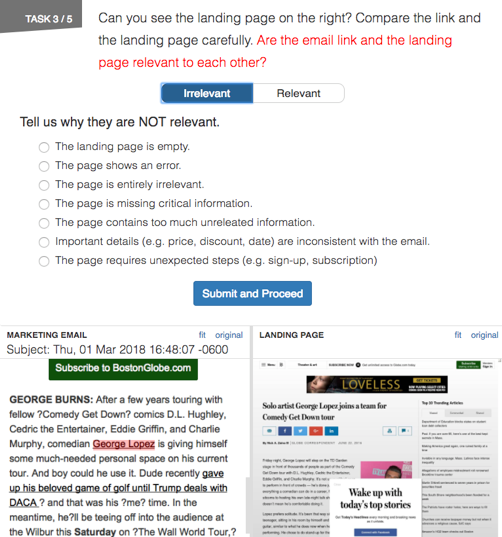
\includegraphics[width=1.0\columnwidth]{figures/mturk-screen}
  \caption{A web-based experimental platform for collecting link relevance labels. Participants cross-check a link (highlighted in red) in a marketing email (bottom left) and its landing page (bottom right). They voted the link to be either relevant or irrelevant, and chose the best reason among common types of misalignments.}~\label{fig:mturk-screen}
\end{figure}


\begin{figure}[tbp]
  \centering
  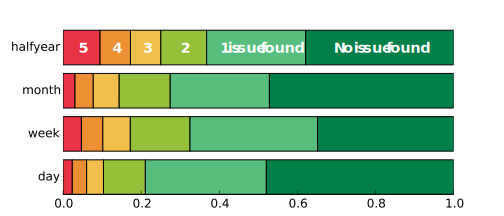
\includegraphics[width=1.0\columnwidth]{figures/vote-dist}
  \caption{Links in the emails that were received within three days are perceived to be more relevant than older emails. Every link was evaluated five times. The portions in red indicate the percentages of links that all the participants found misalignment issues. The portions in green passed with no issue.}~\label{fig:vote-dist}
\end{figure}



\begin{table}
  \small
  \centering
  \begin{tabular}{l r r r | r r}
    % \toprule
    & & \multicolumn{2}{c}{\small{\textit{\# links per email}}} & \multicolumn{2}{c}{\small{\textit{\# issues per link}}} \\
    {\small\textit{Email Group}}     & {\small \textit{\# emails}}   & {\small \textit{Avg.}} & {\small \textit{Std.}} & {\small \textit{Avg.}} & {\small \textit{Std.}}\\
    \midrule
    Day (0-3 days old)          & 40    & 27.3  & 15.5  & 0.18  & 0.24\\
    Week (7-10 days)            & 40    & 29.2  & 20.8  & 0.26  & 0.28\\
    Month (30-33 days)          & 38    & 28.2  & 20.2  & 0.21  & 0.27\\
    Half year (180-183)         & 35    & 26.8  & 26.6  & 0.30  & 0.33\\
    \midrule
    Overall                     & 153    & 27.9  & 21.0 &  0.24 & 0.28\\
    % \bottomrule
  \end{tabular}
  \caption{Four groups of emails that we collected link relevance labels. The \# emails are less than 40 for Month and Half year groups because some of images were not loading in seven emails.}~\label{tab:email_groups}
\end{table}


\subsection{Result}
Total 4266 workers from MTurk participated the experiment. Their ages were average 31.2 (\textit{MED} = 28, \textit{STD} = 9.4)  57.1\% of them were male, and 42.9\% were female. % Male:2434, Female:1832

\subsubsection{Perceived Relevance of Links}
Each link was evaluated by five participants. For the ground-truth relevance score of each link, we use \textit{the number of issues} found by five participants. For instance, an obviously misaligned link would have five issues perceived by participants. A perfectly relevant link would have no issue at all. As illustrated in Figure~\ref{fig:vote-dist}, five stacked bars from left (red) to right (green) represent how many emails in each group were evaluated to be completely irrelevant (five issues) to relevant (no issue). 

We expected to see decay of link relevance over time, which turns out to be partially true. The "day" group has the smallest (26 emails; 2.4\%) amount of links having five issues (i.e. 24 emails in red box), and the largest (523 emails; 47.9\%) of links having no issue. In contrast, the "half year" group as the largest (89; 9.5\%) amount of links having five issues, and the smallest (355; 37.8\%) amount of links having no issue. However, the "week" group turns out to be worse than the "month" group. Overall, a Kruskal-Wallis H test showed that there was a significant statistical difference between the four groups (\textit{H} = 80.1, \textit{p} < 0.001), and Mann-Whitney U posthoc comparisons after Bonferroni correction show that the "day" group is significantly more relevant to the "month" group than to the "week" and "half year" groups (\textit{p} < 0.001). Also the "half year" group is worse than the "month" group (\textit{p} < 0.001)    


\begin{figure}[tbp]
  \centering
  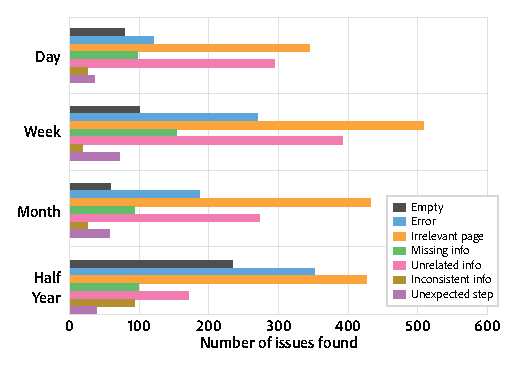
\includegraphics[width=1.0\columnwidth]{figures/issues_group}
  \caption{\c{Irrelevant page} is the most frequent type of misalignment for any group. Older emails in the "half year" group received more reports of \c{empty}, \c{error} pages, and \c{inconsistent info}. However, the number of \c{unrelated info} is significantly more common for the "week" group.}~\label{fig:issues_group}
\end{figure}


\subsubsection{Perceived Types of Misalignments}
The most common type of misalignment is \c{Irrelevant Page} (reported 1712 times), followed by \c{unrelated info}(1131), \c{error}(929), \c{empty}(472), \c{missing info}(443), \c{unexpected step}(203), and \c{inconsistent info}(162). The "day" group contains the smallest(999) number of misalignments. In contrast, the "week" group had 1513 misalignments reported, which is even larger than the "half year" group (1414). Figure~\ref{fig:issues_group} provides the numbers broken into different groups. There was a significant difference between distributions of misalignments across groups (${\chi}^2$ = 376.2, $p < 0.001$). For instance, the "half year" group has \c{empty}, \c{error}, and \c{inconsistent info} more frequently compared to emails in the other groups ($p < 0.001$). However, \c{unrelated info} was reported more frequently for emails in the "week" group ($p < 0.001$). 

% OVERALL TYPES OF MISALIGNMENTS: {u'inconsistent_info': 162, u'unexpected_step': 203, u'missing_info': 443, u'unrelated_info': 1131, u'unrelated_page': 1712, u'error': 929, u'empty': 472}

% TYPES BY GROUP: {'week': {u'inconsistent_info': 18, u'unexpected_step': 71, u'unrelated_info': 392, u'missing_info': 153, u'unrelated_page': 509, u'error': 270, u'empty': 100}, 'halfyear': {u'inconsistent_info': 93, u'unexpected_step': 39, u'missing_info': 99, u'unrelated_info': 171, u'unrelated_page': 426, u'error': 352, u'empty': 234}, 'day': {u'inconsistent_info': 25, u'unexpected_step': 36, u'missing_info': 98, u'unrelated_info': 295, u'unrelated_page': 345, u'error': 121, u'empty': 79}, 'month': {u'inconsistent_info': 26, u'unexpected_step': 57, u'unrelated_info': 273, u'missing_info': 93, u'unrelated_page': 432, u'error': 186, u'empty': 59}}


% Chi-Square contingency table (376.19091535578804, 8.307230515268001e-69, 18, array([[ 93.33491686, 183.70368171, 338.5368171 ,  87.60035629,
%         223.64786223,  32.03444181,  40.14192399],
%       [141.3570863 , 278.22189232, 512.7189232 , 132.67201108,
%         338.71793349,  48.51662708,  60.79552652],
%       [105.20031671, 207.05740301, 381.57403009,  98.73673793,
%         252.07957245,  36.10688836,  45.24505146],
%       [132.10768013, 260.01702296, 479.17022961, 123.9908947 ,
%         316.55463183,  45.34204276,  56.81749802]]))




%http://patorjk.com/software/taag/#p=display&f=ANSI%20Shadow&t=METRIC
% ███╗   ███╗███████╗████████╗██████╗ ██╗ ██████╗
% ████╗ ████║██╔════╝╚══██╔══╝██╔══██╗██║██╔════╝
% ██╔████╔██║█████╗     ██║   ██████╔╝██║██║     
% ██║╚██╔╝██║██╔══╝     ██║   ██╔══██╗██║██║     
% ██║ ╚═╝ ██║███████╗   ██║   ██║  ██║██║╚██████╗
% ╚═╝     ╚═╝╚══════╝   ╚═╝   ╚═╝  ╚═╝╚═╝ ╚═════╝
\section{LINK RELEVANCE METRIC}
The key component of our system is the link relevance metric. Given a link and its landing page, our task is to predict if customers perceive the landing page misaligned. 
%We assume the link is an anchor tag in the HTML code of an email. 
We approach this problem using both unsupervised, i.e.\,cosine similarity in combination with vector space models, as well as deep neural network models. 

Figure~\ref{fig:model_baseline} shows the precision, recall, and F-scores of two unsupervised baseline models applied to three different classification settings. The number of votes required to define the target class distinguishes the classification problems. Both baseline models compute the cosine similarity between a landing page and a concatenation of the link text, its corresponding email body, and the subject line. If the similarity score is lower than a given threshold, the landing page is considered misaligned. The first model is based on a TFIDF vector space model while the second one uses the Universal Sentence Encoder from Tensorflow in order to compute a $512$-dimensional text embedding as described in~\cite{cer_2018}. Increasing the number of votes required for the target class is decreasing the number of target instances, which changes the class balance. The $x$-axis represents a classification threshold for the cosine similarity scores. If the threshold is set to one, the precision score reflects the class balance. The recall curve provides information about the distribution of similarity scores in the target class. Analogous, the precision curve shows distribution of similarities in the non-target class.

For our study we define three settings with different voting thresholds that determine our ground-truth. The number of votes for the target class label "misaligned" is defined by the number of people that indicated an issue with the landing page in the MTurk survey. For a minimum risk setting we consider one or more votes sufficient for the target class, for majority voting we require at least 3 votes, and for complete agreement we require 5 votes.

\begin{figure}[bt]
	\centering
	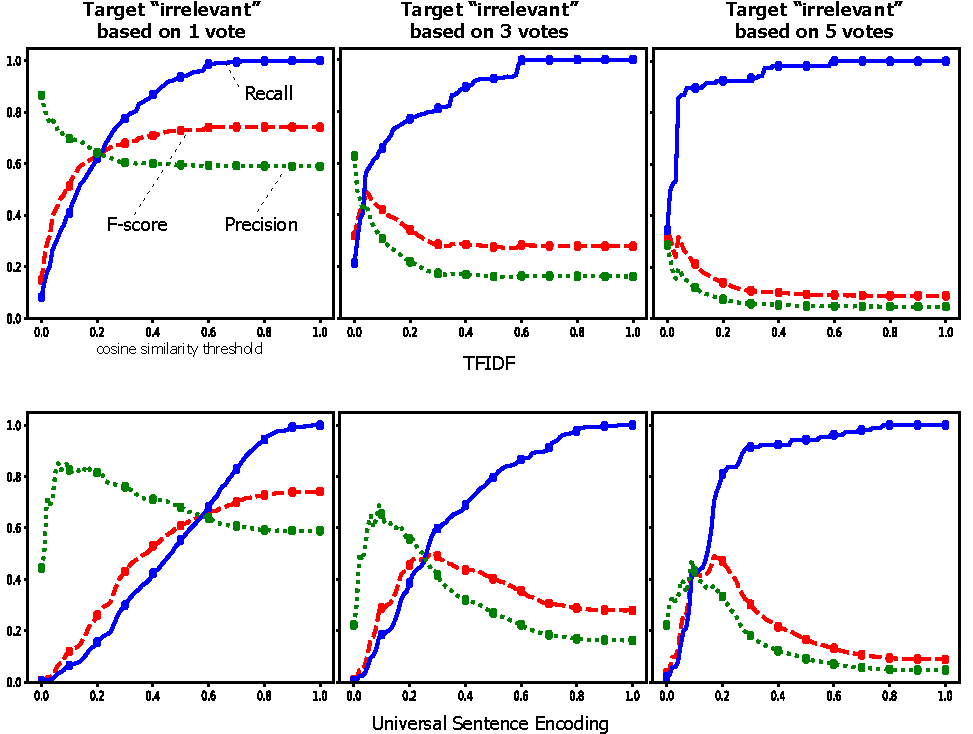
\includegraphics[width=1.0\columnwidth]{figures/cos_sim_link_text_email_subject_email_text_votes_1_3_5.pdf}
	\caption{Baseline precision, recall, and F-scores for two unsupervised models and different problem parameters.}
	\label{fig:model_baseline}
\end{figure}

We study variations of two feedforward deep learning architectures for classification. All of the models combine features based on the landing page content with different sets of features representing the link and its email context. Out of experiments with TFIDF, term frequencies, and term occurrences we report results based on binary term occurrence vectors, which lead to the best effectiveness on the test sets. In order to represent a link, we combine the anchor text of the link with extracted OCR information and image tags in case an image has been available. We are using the Google Tesseract OCR engine~\cite{smith_2007} and the Inception V3 model~\cite{szegedy_2015} for these tasks. Furthermore, the subject line and the body of the email that includes the corresponding link can be input to the proposed models. We report the combinations of inputs that lead to the highest F-score. 

Figure~\ref{fig:model_a_b} shows variations of a simple deep learning architecture. Each input in variation~(a) has a lower dimensional distributed representation with rectifiers as activation functions and dropout. As illustrated, each input uses an individually fitted, lower cased vocabulary in order to map text to a numeric vector space. It follows another dense layer with rectified linear units before the output layer. Variation~(b) differs in terms of the input embedding which is inferred by employing the pre-trained Unified Sentence Encoder~\cite{cer_2018}.

\begin{figure}[t]
	\centering
	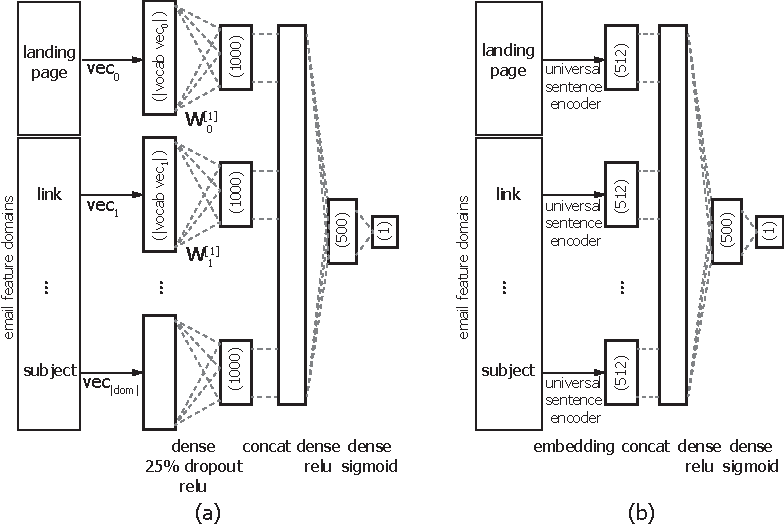
\includegraphics[width=1.0\columnwidth]{figures/model_0_4_1_and_6.pdf}
	\caption{Two variations of a simple feedforward deep learning architecture. Inputs are landing page and various link features, whereby (a) uses term occurrences and individual vocabularies per feature domain and (b) a pre-trained text embedding.} %~\cite{cer_2018}
	\label{fig:model_a_b}
\end{figure}

Figure~\ref{fig:model_c} aims to model the semantic difference between a link and its landing page by computing element-wise differences and multiplications. Therefore, the vocabulary as well as the embedding weights of the first fully connected layer are shared across all inputs. It follows a lower dimensional dense layer with rectified linear units and the output layer as before.

\begin{figure}[t]
	\centering
	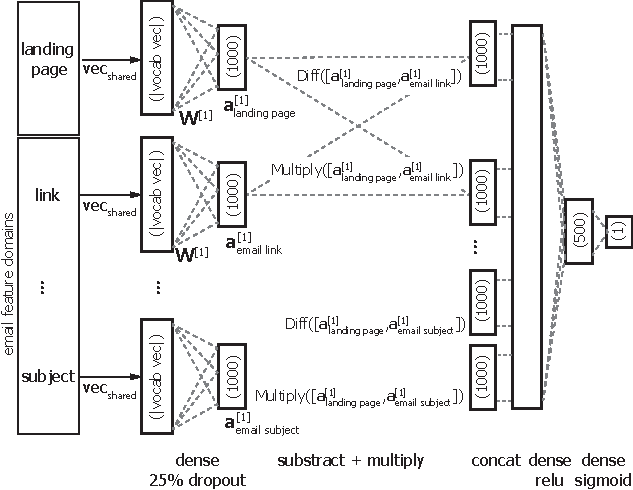
\includegraphics[width=1.0\columnwidth]{figures/model_0_6.pdf}
	\caption{A deep learning architecture that uses shared embedding weights and models the differences between email and landing page features using subtraction and multiplication layers.}
	\label{fig:model_c}
\end{figure}

Table~\ref{tab:effectiveness} summarizes precision, recall, and F-scores for the proposed architectures. It reports the combination of link inputs that results in the highest F-score for each architecture. The experiments use an early stopping criteria based on the validation loss as generalization strategy. For model fitting we employ binary cross entropy as loss function, balanced class weights, and the Adam optimization algorithm~\cite{kingma_2014}.

\begin{table}[bt]
	\small
	\centering
	\begin{tabular}{l r r r}
		{\centering\textbf{Model}}   &  \textbf{F}  & \textbf{Prec} &  \textbf{Rec}\\
		\midrule
		\multicolumn{4}{c}{\textit{Target class requires at least 1 vote}}\\
    	\midrule
		Figure \ref{fig:model_a_b}(a), link + subject line & $^*$\textbf{0.76} & 0.63 & 0.95\\ %model_0_4_2
		%                                                   & 0.59 & $^{**}$0.81 & 0.46\\
   		Figure \ref{fig:model_a_b}(b), link + subject line + email body & $^*$0.75  & 0.60  & 0.99\\%model_6
   		%   		                                                   & 0.71 & $^{**}$0.74   & 0.69\\%model_6
		Figure \ref{fig:model_c}, link + subject line + email body & $^*$0.74 & 0.72 & 0.76\\%model_0_6
		%                                                      & 0.74& $^{**}$0.72   & 0.76\\%model_0_6
		\midrule			                                        
		\multicolumn{4}{c}{\textit{Target class requires at least 3 votes}}\\
		\midrule		
		Figure \ref{fig:model_a_b}(a), link + subject line + email body & $^*$0.63 & 0.76 & 0.54\\ %model_0_4_1
		%							                               & 0.39 & $^{**}$0.90 & 0.25\\
        Figure \ref{fig:model_a_b}(b), link & $^*$0.43 & 0.65  & 0.33\\%model_6_1
		%	                                     & 0.49 & $^{**}$\textbf{0.96}   & 0.15\\%model_6_1
		Figure \ref{fig:model_c}, link + subject line & $^*$\textbf{0.66} & 0.78  & 0.57\\
		%                                              & 0.45 & $^{**}$0.89 & 0.30\\
		\midrule			                             
		\multicolumn{4}{c}{\textit{Target class requires at least 5 votes}}\\
		\midrule		
		Figure \ref{fig:model_a_b}(a), link + subject line + email body & $^*$0.59& 0.69 & 0.51\\ %model_0_4_1_1
		%						                                   & 0.59 & $^{**}$\textbf{0.69} & 0.51\\ %model_0_4_1_1
		Figure \ref{fig:model_a_b}(b), link & $^*$0.46 & 0.50 & 0.42\\%model_6_1
   		%			                             & 0.46 & $^{**}$0.50 & 0.42\\%model_6_1
		Figure \ref{fig:model_c}, link & $^*$\textbf{0.63} & 0.56  & 0.72\\%model_10_2
		%			                        & 0.63 & $^{**}$0.56 & 0.72\\%model_10_2
	\end{tabular}
	\caption{The table reports the best performing deep learning models according to its F-score on a held out test set.}
	\label{tab:effectiveness}
\end{table}

 %For example, imagine a link containing "offer" and a landing page containing "deal". Even though the two words are semantically similar, vector models would count them completely unrelated. Word embedding is a popular method that distributes each word into a fixed-dimensional vector space

In the minimum risk setting that requires at least one vote for the target class, the neural network architectures described in Figure~\ref{fig:model_a_b} achieve the best recall and F-scores. However, in comparison to our unsupervised baselines, the neural networks are not significantly better. For settings that require more votes, our architecture illustrated in Figure~\ref{fig:model_c} produces the best results. 

%The process consists three steps - feature selection, vector processing, and similarity measure. Since there are many options for each step, we compared variations of them to find the best combination. 

%\subsubsection{Feature Selection}
%The first step of calculating link relevance is to extract a feature vector from the email. The vector should be able to characterize what people would expect when clicking the link. The entire email may not be an ideal option since it might have lots of unrelated information. In contrast, the link alone tend to lack contextual information. For example, when users click a 'buy' button, he/she would expect to see a specific product next to the button at the landing page. 

%\subsubsection{Image Features}
%Links are not always text but also include images often. In that case, we can extract crucial information from link images. We use Tesseract OCR library  to extract text in image files. We also extracted concept of images by using ImageNet , a pre-trained Tensorflow library.  

%\subsubsection{Word Embedding}
%Vectors of short messages such as links tend to be very noisy and sparse in their use of vocabulary. For example, imagine a link containing "offer" and a landing page containing "deal". Even though the two words are semantically similar, vector models would count them completely unrelated. Word embedding is a popular method that distributes each word into a fixed-dimensional vector space [2]. There are three   
%\subsubsection{Vector Similarity Measure}
%Given two vectors of a link and a landing page, the metric needs to calculate a similarity score. While there is a large number of similarity measures, we use cosine similarity which is the most widely used one.

%\subsection{Evaluation of Model Prediction}
%In this section we compare performance of various settings of link relevance metric. 


% ███╗   ███╗ ██████╗ ███╗   ██╗██╗████████╗ ██████╗ ██████╗ ██╗███╗   ██╗ ██████╗ 
% ████╗ ████║██╔═══██╗████╗  ██║██║╚══██╔══╝██╔═══██╗██╔══██╗██║████╗  ██║██╔════╝ 
% ██╔████╔██║██║   ██║██╔██╗ ██║██║   ██║   ██║   ██║██████╔╝██║██╔██╗ ██║██║  ███╗
% ██║╚██╔╝██║██║   ██║██║╚██╗██║██║   ██║   ██║   ██║██╔══██╗██║██║╚██╗██║██║   ██║
% ██║ ╚═╝ ██║╚██████╔╝██║ ╚████║██║   ██║   ╚██████╔╝██║  ██║██║██║ ╚████║╚██████╔╝
% ╚═╝     ╚═╝ ╚═════╝ ╚═╝  ╚═══╝╚═╝   ╚═╝    ╚═════╝ ╚═╝  ╚═╝╚═╝╚═╝  ╚═══╝ ╚═════╝ 
                                                                                 
%  █████╗  ██████╗ ███████╗███╗   ██╗████████╗                                     
% ██╔══██╗██╔════╝ ██╔════╝████╗  ██║╚══██╔══╝                                     
% ███████║██║  ███╗█████╗  ██╔██╗ ██║   ██║                                        
% ██╔══██║██║   ██║██╔══╝  ██║╚██╗██║   ██║                                        
% ██║  ██║╚██████╔╝███████╗██║ ╚████║   ██║                                        
% ╚═╝  ╚═╝ ╚═════╝ ╚══════╝╚═╝  ╚═══╝   ╚═╝  

\section{Intelligent Monitoring Agent}
We now introduce the intelligent monitoring agent for promotion links. It enables marketers to efficiently monitor links in their promotion emails in terms of relevance with landing pages. Figure~\ref{fig:pipeline} shows an overview of the system. The pipeline begins by (a) a marketer registering an email to the agent. The document analyzer extracts rendered text, links (i.e. anchor tags), and images within each anchor tag. Extracted information is stored in the database.

\subsection{Periodic Evaluation of Link Relevance}
The scheduler periodically triggers the headless browser to retrieve current content (i.e. text and screenshot) of all the landing pages stored in the database. Then the relevance metric predicts whether each pair of link and landing page contains misalignment. Lastly, the report generator notifies the marketer about any potential misalignments. The entire process updates the database so that the marketer can see the current overview and previous reports.  

\begin{figure}
\centering
  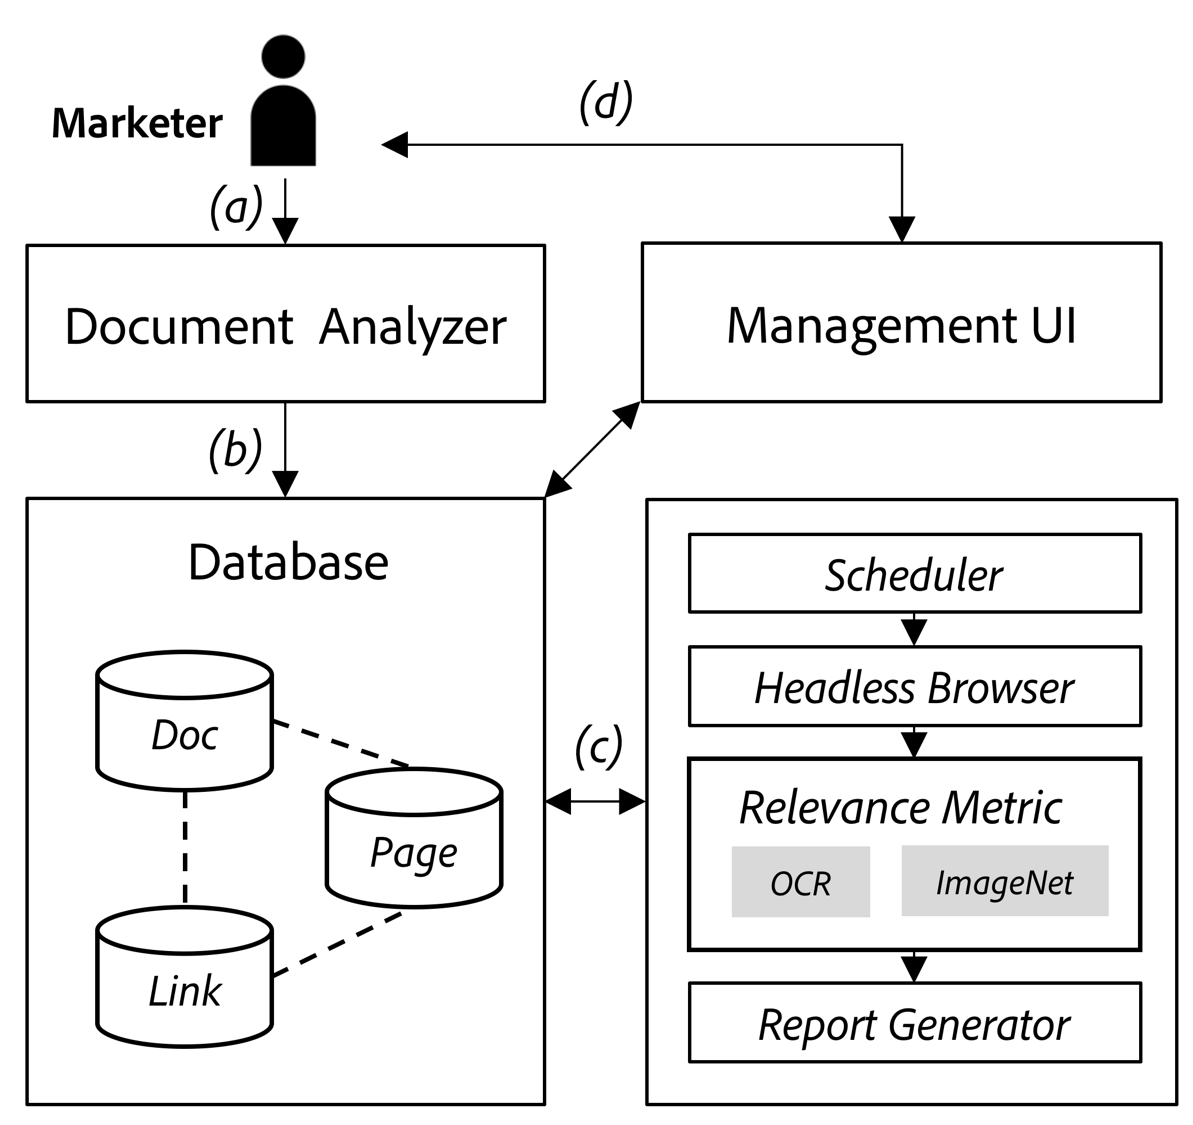
\includegraphics[width=0.8\columnwidth]{figures/pipeline}
  \caption{The pipeline of monitoring link relevance. As a marketer (a) registers a promotion email, (b) the document analyzer extracts links and other information, and stores in the database. (c) The scheduler periodically triggers the headless browser to retrieve content of all the registered landing pages. Then the relevance metric calculates relevance of each pair of link and landing page. The report generator notifies the owner about potentially misaligned links. (d) The marketer can use the manager UI to overview his/her documents and recent reports.}~\label{fig:pipeline}
\end{figure}

\begin{figure}[tbp]
\centering
  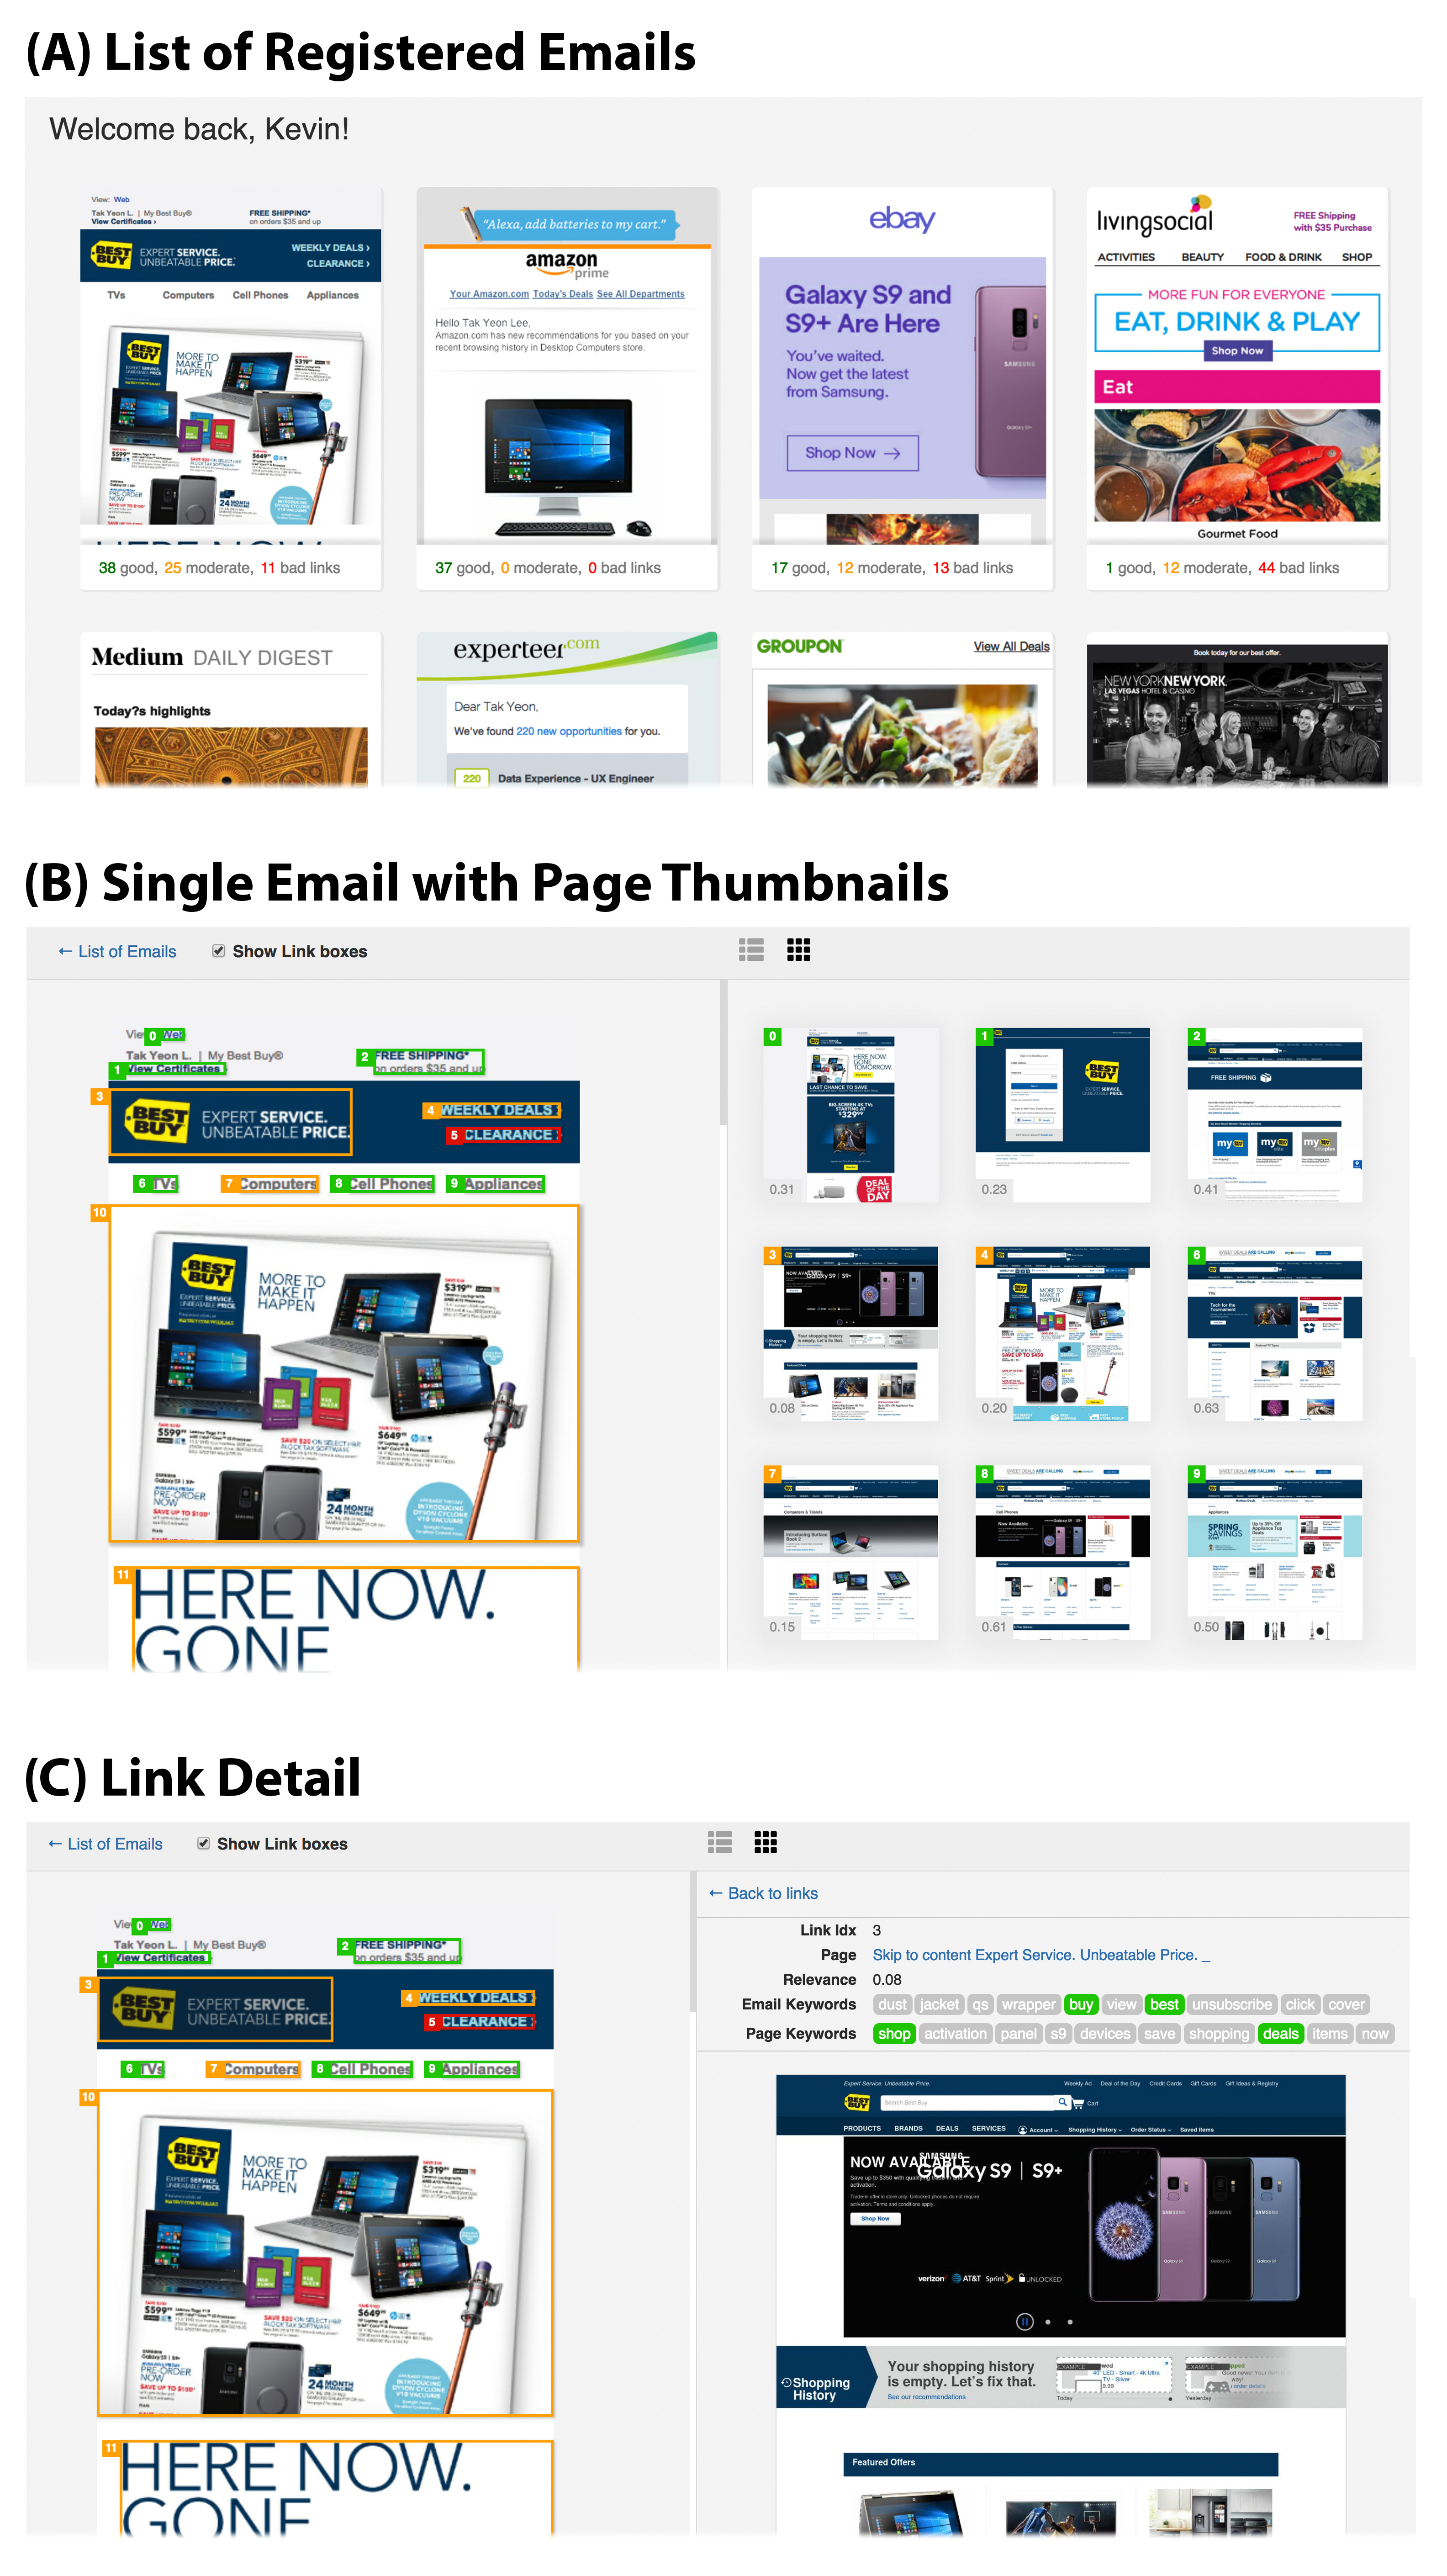
\includegraphics[width=\columnwidth]{figures/system-screenshots}
  \caption{The management UI consists of three screens. In A, marketers can overview status of their registered emails quickly. By clicking a thumbnail image in A, marketers can review all the landing pages of the emails in B. By clicking a rectangle around a link on the left panel of B, or by clicking a landing page thumbnail, marketers can see detailed information in C.}~\label{fig:system-screenshots}
\end{figure}


\subsection{Management UI}
The management UI of the system allows marketers to monitor current status of their emails, and review the latest report.    

%  (A) shows thumbnail images of the emails registered by the marketer, with the numbers of good, moderate, and bad links. (B) shows a single email (left panel) and thumbnail images of its landing pages. Green, orange, and red rectangles indicate estimated relevance (good, moderate, and bad respectively) of each pair of link and landing page. (C) provides the most detailed information of a link and its landing page. Relevance score and Email / Page keywords help marketers understand the estimated relevance. 


\subsubsection{List of Registered Emails}
Email marketers would create a number of emails regularly. As an overview of all the previously registered emails, Figure~\ref{fig:system-screenshots} (A) is created. Each thumbnail icon is a screenshot of an email with numbers of how many good, moderate, and bad links (e.g. {\color{green}37} good, {\color{orange}25} moderate, {\color{red}11} bad links) the latest report found in the email.  

\subsubsection{Single Email with Landing Page Thumbnails}
During the data collection, we observed that a single promotion email may have over 100 links. To enable marketers to efficiently review a large number of links and landing pages, Figure~\ref{fig:system-screenshots} (B) provides two panel UI. In the left panel, the screenshot of the email is shown. It also shows rectangles over each link, which can be toggled by clicking "Show Link Box". The boxes have either green, orange, and red colors based on their estimated relevance score. For instance, links of green boxes are likely to be relevant to landing pages, while links of red boxes might be misaligned. Orange indicates moderate relevance, which requires the marketer's validation. The threshold of the color scheme is not fixed or trained yet, but customized by the marketer. The right panel lists screenshots of all the landing pages of the email. Screenshots have index numbers in green, orange, and red colors that correspond to links in the left panel. Marketers can click a link box or a screenshot to see more detailed information. 

\subsubsection{Link Detail}
Since the link relevance can be subjective specially in moderate cases, the metric provides suggestive notifications that require marketers to validate each issue and decide how to address. Thus marketers might need details about individual landing pages and why the link is a potential issue. Figure~\ref{fig:system-screenshots} (C) shows an actual relevance score (i.e. the probability of the link to be perceived misaligned) and top-10 keywords of email and page. The keywords are 10 words with the highest TF-IDF values in the email vector and the page vector. Some keywords are highlighted in green, which means that the keyword exists in top-100 keywords of the other vector. For instance, "buy" and "best" in the email keyword, and "show" and "deals" in the page keywords of Figure~\ref{fig:system-screenshots} (C) make the link more relevant. In contrast, other keywords in gray represent that they only exist in one side. 



%  ██████╗ █████╗ ███████╗███████╗    ███████╗████████╗██╗   ██╗██████╗ ██╗   ██╗
% ██╔════╝██╔══██╗██╔════╝██╔════╝    ██╔════╝╚══██╔══╝██║   ██║██╔══██╗╚██╗ ██╔╝
% ██║     ███████║███████╗█████╗      ███████╗   ██║   ██║   ██║██║  ██║ ╚████╔╝ 
% ██║     ██╔══██║╚════██║██╔══╝      ╚════██║   ██║   ██║   ██║██║  ██║  ╚██╔╝  
% ╚██████╗██║  ██║███████║███████╗    ███████║   ██║   ╚██████╔╝██████╔╝   ██║   
%  ╚═════╝╚═╝  ╚═╝╚══════╝╚══════╝    ╚══════╝   ╚═╝    ╚═════╝ ╚═════╝    ╚═╝   


\section{LONGITUDINAL CASE STUDY}
Along the iterative development process, we regularly demonstrated the system and conducted case study with real email marketers in a company. They provided us insightful feedback and suggestions via regular meetings throughout 8 months period. 

\subsubsection{Efficiency is an obvious benefit}
Email marketers told us that they usually test important links once or twice before sending out. After deployment, they rarely test links. They found thumbnails of all the landing pages (Figure~\ref{fig:system-screenshots}.B) with color highlights indicating link relevance will increase the efficiency of link testing to a great extent.  

\subsubsection{Lack of Interpretability}
When marketers saw potential misalignments in the report, they tried to understand the reason why the metric estimated. Although email / page keywords in Figure~\ref{fig:system-screenshots}.C were helpful, marketers often told us that some results are difficult to understand.      

\subsubsection{Controllability with Efficiency}
Since results of the relevance metric may not always be perfectly accurate, marketers wanted to get more controls. For instance, they want to white list specific links or landing pages so that the agent will skip testing them in future. The threshold of good, moderate, and bad links is another setting that marketers want to have control over. They also wondered how frequently the system will check each landing page, and how they can manage the setting.  
Nevertheless, marketers also acknowledged that having too many controls would make the testing process inefficient.  

\subsubsection{Scalable to monitor a large number of similar emails} 
Corporate marketers told us that they often create a large number of similar emails for multiple languages, locations, browsers, A/B testing, and special content for target segments. The list of registered emails needs to group them automatically. Misalignments found from similar emails should be bundled so that marketers can efficiently handle them.

\subsubsection{Additional custom tests} 
While we focused on testing content relevance, marketers regularly do additional tests. For instance, URLs of promotion links often contain special parameters for tracking. Marketers should make sure such parameters exist in the landing page URLs.    


\section{Limitation and Future Work}
As the first step toward the problem, our work has many limitations. First, participants of our survey and experiments were recruited from Mturk, which may not precisely represent the population of Internet users. For more generalizable outcome, we will also collect data from different participant pools, and perform cross-validation. Similarly, we collected labeled data of links within 160 promotion emails, which many not represent the entire spectrum of online documents. In future we will apply a similar approach to other types of documents such as web pages, wiki or PDF documents. 

Although we collected positive feedback from our longitudinal case study, a comprehensive and controlled user study will be able to assess the actual benefits of our system. We will also add more features requests by the marketers as discussed in the above section. 

% \begin{itemize}
%     \item Ideally the four groups of emails should be under a longitudinal setting. In other words, we need to pick an email and keep monitoring how its link relevance change over time.   
%     \item ...  
% \end{itemize}


\section{Conclusions}
In this paper we presented a novel method for efficiently monitoring relevance of links and their landing pages. Along the development process, we identified types of common misalignments as result of an online survey. We then collected labeled training data, and experimented a wide range of link relevance metric to find the best performing metric. We developed the monitoring agent including the management UI that enables marketers to monitor current status of their emails, and validate potential misalignments. Finally, results of a longitudinal case study with corporate marketers suggest that our method would provide benefits for them to efficiently run email campaigns by testing and tracking link relevance of promotional emails. 


% BALANCE COLUMNS
\balance{}

% REFERENCES FORMAT
% References must be the same font size as other body text.
\bibliographystyle{SIGCHI-Reference-Format}
\bibliography{int_uist}

\end{document}

%%% Local Variables:
%%% mode: latex
%%% TeX-master: t
%%% End:
